\documentclass[10pt]{extarticle}
\title{}
\author{Avinash Iyer}
\date{}

%font setup
%
%\usepackage[math]{anttor}

%paper setup
\usepackage{geometry}
\geometry{letterpaper, portrait, margin=1in}
\usepackage{fancyhdr}

%symbols
\usepackage{amsmath}
\usepackage{amssymb}
\usepackage{hyperref}
\usepackage{gensymb}

\usepackage[T1]{fontenc}
\usepackage[utf8]{inputenc}

%chemistry stuff
\usepackage[version=4]{mhchem}
\usepackage{chemfig}

%plotting
\usepackage{pgfplots}
\usepackage{tikz}

%\usepackage{natbib}

%graphics stuff
\usepackage{graphicx}
\graphicspath{ {./images/} }

%a useful command
\newcommand{\plain}[1]{\textrm{#1}}

%code stuff
%when using minted, make sure to add the -shell-escape flag
%you can use lstlisting if you don't want to use minted
%\usepackage{minted}
%\usemintedstyle{pastie}
%\newminted[javacode]{java}{frame=lines,framesep=2mm,linenos=true,fontsize=\footnotesize,tabsize=3,autogobble,}
%\newminted[cppcode]{cpp}{frame=lines,framesep=2mm,linenos=true,fontsize=\footnotesize,tabsize=3,autogobble,}

\usepackage{listings}
\usepackage{color}
\definecolor{dkgreen}{rgb}{0,0.6,0}
\definecolor{gray}{rgb}{0.5,0.5,0.5}
\definecolor{mauve}{rgb}{0.58,0,0.82}

\lstset{frame=tb,
	language=Java,
	aboveskip=3mm,
	belowskip=3mm,
	showstringspaces=false,
	columns=flexible,
	basicstyle={\small\ttfamily},
	numbers=none,
	numberstyle=\tiny\color{gray},
	keywordstyle=\color{blue},
	commentstyle=\color{dkgreen},
	stringstyle=\color{mauve},
	breaklines=true,
	breakatwhitespace=true,
	tabsize=3
}
\pagestyle{fancy}
\fancyhf{}
\rhead{Avinash Iyer, Tobias Searcy-Jorgensen}
\lhead{Lab 9: Simple Harmonic Motion (Pendulum)}
\begin{document}{
\section*{Abstract}
In this experiment, we analyzed the effects of varying different quantities intrinsic to a pendulum in order to find which ones had substantial effects on the period of the pendulum. In Experiment 1, we measured out different lengths on the string while maintaining a starting angle of 10$^{\circ}$ and a bob mass of $31.2$ grams. These varying lengths produced a wide variety of periods on the pendulum. In Experiment 2, we varied the starting angle of the pendulum while maintaining a length of $0.5$ meters and mass of $31.2$ grams. Up to a point, the periods were quite consistent, but when the angle increased to $80^{\circ}$, the period was substantially higher. In Experiment 3, we varied the mass of the pendulum bob while maintaining a length of $0.5$ meters and a starting angle of $10^{\circ}$, finding a very consistent set of period measurements. After performing these experiments, we calculated $g$ by regressing the square of the period against the length, then dividing the resultant sum by $4\pi^2$, then taking its inverse in order to find an experimental value for the acceleration due to gravity, which we found was $9.8\pm 0.3$ m/s$^2$. These results were consistent with the theory surrounding the effects of changing various quantities on the pendulum's period. 
\section*{Methods}
In order to examine the effects of changing various quantities on the period of the pendulum, we worked with a setup as follows:
  \begin{itemize}
    \item Rod with a hole which a string is threaded through.
    \item Varying number of washers whose masses are measured.
    \item Protractor attached to the rod which is used to measure the angle of the string. 
  \end{itemize}
With this setup, we are able to vary the measurement of the length of the string, the angle of the string, and the mass of the pendulum bob. A representation is shown below.
  \begin{center}
    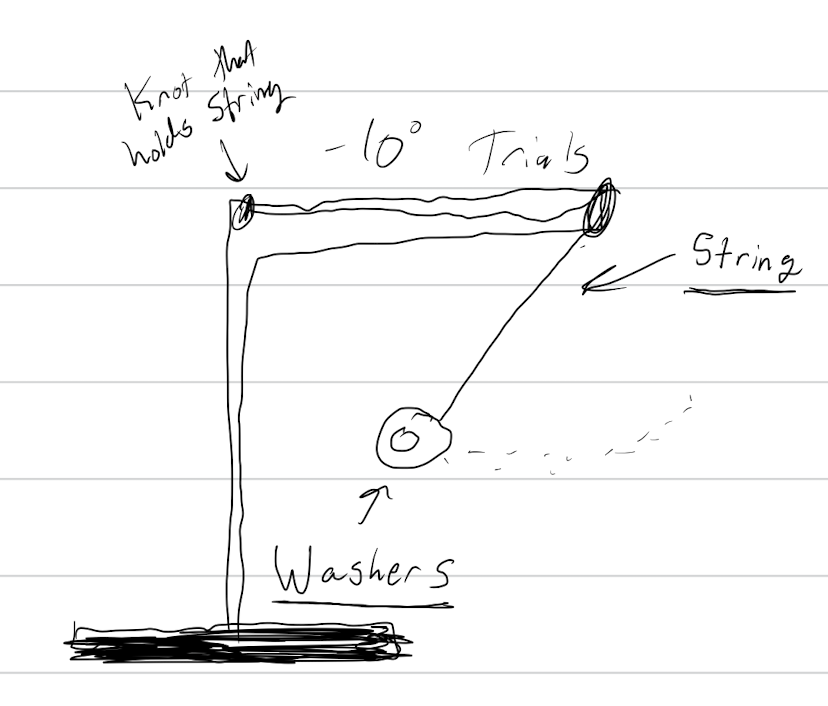
\includegraphics[width=10cm]{Lab9Image1} \\
    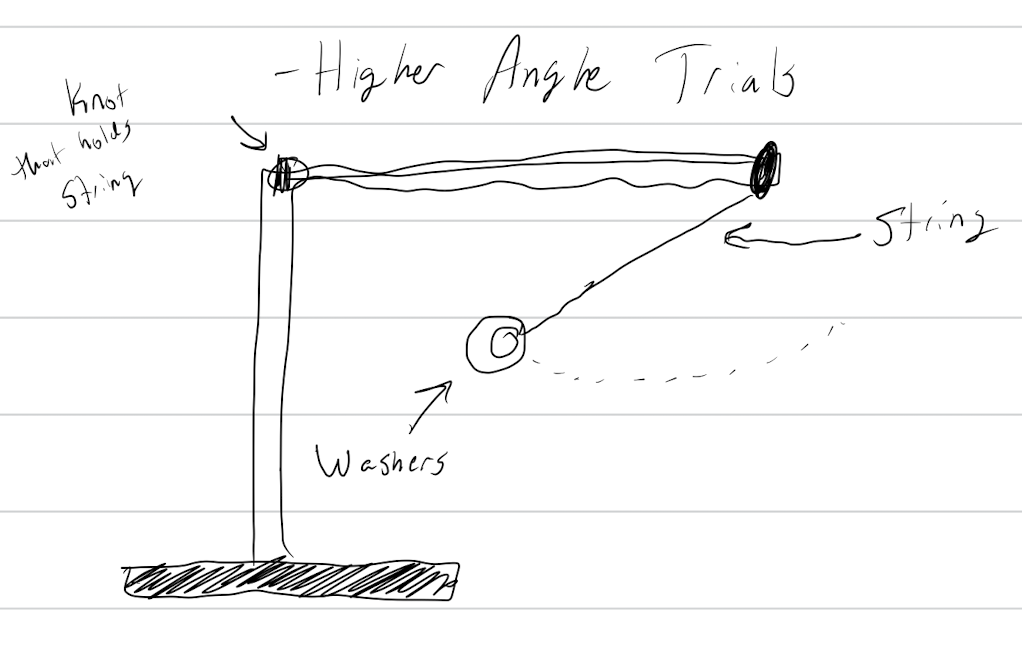
\includegraphics[width=10cm]{Lab9Image2}
  \end{center}
One lab member will release the pendulum and simultaneously start a stopwatch while measuring out ten periods of the pendulum. After measuring out ten periods, the other lab partner will enter the values into the spreadsheet. The participants will hold two of $\{$Angle, Mass, Length$\}$ constant during a set of trials. Experiment 1 will vary the length of the pendulum, Experiment 2 will vary the angle of the string, and Experiment 3 will vary the mass of the pendulum bob.\\
\\
Errors in the lab can be identified as follows:
  \begin{itemize}
    \item Measurement of the various lengths of the string during the trials in which length is varied.
    \item Measurement of the angles during the trials in which the angle is varied.
    \item Instrumental uncertainty in the mass of the washers. 
  \end{itemize}
 We are assuming that there is no air resistance and negligible friction, as well as zero mass in the string.
\section*{Data Results and Analysis}
\subsection*{Experiment 1}
\begin{center}
	\renewcommand{\arraystretch}{1.5}
	\begin{tabular}{c|c}
	Quantity & Value\\
	\hline
	Number of Washers & 5\\
	Mass of Washers (g) & $31.2\pm 0.1$ \\
	Starting Angle of String & $10^{\circ}$
	\end{tabular}\\
	\vspace*{10pt}
	\begin{tabular}{c|c|c|c|c}
		Length of string (m) & $10T$ (s) & $T$ (s) & $\delta (10T)$ (s) & $\delta T$ (s) \\
		\hline
		$1.00\pm 0.01$ & $20.00$ & $2.000$ & $0.3$ & $0.03$ \\
		$0.90\pm 0.01$ & $19.06$ & $1.906$ & $0.3$ & $0.03$ \\
		$0.80\pm 0.01$ & $17.62$ & $1.762$ & $0.3$ & $0.03$ \\
		$0.70\pm 0.01$ & $16.66$ & $1.666$ & $0.3$ & $0.03$ \\
		$0.60\pm 0.01$ & $15.41$ & $1.541$ & $0.3$ & $0.03$ \\
		$0.50\pm 0.01$ & $14.18$ & $1.418$ & $0.3$ & $0.03$
	\end{tabular}
\end{center}
\subsection*{Experiment 2}%
  \begin{center}
    \renewcommand{\arraystretch}{1.5}
    \begin{tabular}{c|c}
      Quantity & Value\\
      \hline
      Number of Washers & 5\\
      Mass of Washers (g) & $31.2\pm 0.1$ \\
      Length of String (m) & $0.50\pm 0.01$
      \end{tabular}
      \begin{tabular}{c|c|c|c|c}
        Angle ($^{\circ}$) & $10T$ (s) & $\delta (10T)$ (s) & $T$ (s) & $\delta T$ (s) \\
        \hline
        10 & $14.28$ & $0.3$ & $1.428$ & $0.03$\\
        20 & $14.31$ & $0.3$ & $1.431$ & $0.03$ \\
        30 & $14.37$ & $0.3$ & $1.437$ & $0.03$\\
        40 & $14.53$ &  $0.3$ & $1.453$ & $0.03$\\
        50 & $14.81$ & $0.3$ & $1.481$ & $0.03$\\
        80 & $15.85$ & $0.3$ & $1.585$ & $0.03$
        \end{tabular}
    \end{center} 	
\subsection*{Experiment 3}%
  \begin{center}
    \renewcommand{\arraystretch}{1.5}
    \begin{tabular}{c|c}
      Quantity & Value\\
      \hline
      Angle & $10^{\circ}$\\
      Length of String & $0.50\pm 0.01$m
        
    \end{tabular}
    \begin{tabular}{c|c|c|c|c|c}
      Number of Washers & Mass (g) & $10T$ (s) & $T$ (s) & $\delta (10T)$ (s) & $\delta T $ (s)\\
      \hline
      5 & 31.2 & $14.22$ & $1.422$ & $0.3$ & $0.03$ \\
      4 & $25.0$ & $14.19$ & $1.419$ & $0.3$ & $0.03$ \\
      3 & $18.0$ & $14.22$ & $1.422$ & $0.3$ & $0.03$ \\
      2 & $12.5$ & $14.18$ & $1.418$ & $0.3$ & $0.03$ \\
      1 & $6.4$ & $14.25$ & $1.425$ & $0.3$ & $0.03$
      \end{tabular}
  \end{center}
\subsection*{Calculating Acceleration due to Gravity}%
Using the \texttt{LINEST} function in Google Sheets, we get that the slope of $T^2$ versus length is $4.01\pm 0.1$. By the equation $T = 2\pi \sqrt{\frac{l}{g}}$, we get that this slope must be equal to $\frac{4\pi^2}{g}$. By dividing by $4\pi^2$, then taking the inverse, we get a value of $g = 9.8\pm 0.3$. The error on $g$ is found by taking the fractional error  of the slope on the calculated value of $g$.
\section*{Conclusion}
We conclude that the results of the experiment are consistent with the theory that the period of a simple pendulum varies only with length of the pendulum at small angles. Similarly, the calculated value of the acceleration due to gravity is consistent with the theoretical value of the acceleration due to gravity. However, we could expand our experiment further by examining the effects of larger angles on the period of the pendulum beyond the simple $80^{\circ}$ value tested.
}\end{document}
